% !TEX TS-program = pdflatexmk

\documentclass[14pt]{beamer}
\usepackage{newtxtext,newtxmath}
\usepackage{microtype}
\usepackage[english]{babel}
\usepackage{hyperref}
\usepackage{graphicx}
\usepackage{listings}
\lstloadlanguages{Python}
\lstset{language=Python}
\lstset{%
basicstyle=\ttfamily\bfseries,
keywordstyle=\color{blue}, emph={self}, emphstyle={\color{blue}},
identifierstyle=,
commentstyle=\color{brown},
stringstyle=\color{green!50!black},
showstringspaces=false,
emphstyle={[2]\color{purple}},
}
\usepackage{tikz}
\usepackage{pgfplots}
\usepackage{forest}
\usetikzlibrary{calc}
\usetikzlibrary{shapes}
\usetikzlibrary{positioning}
\usetikzlibrary{arrows}
\usepackage{array}
\newcolumntype{L}[1]{>{\raggedright\let\newline\\\arraybackslash\hspace{0pt}}m{#1}}

\mode<presentation>{
\usetheme{Madrid}
\definecolor{uabgreen}{cmyk}{.89,.31,.78,.17}
\usecolortheme[named=uabgreen]{structure}
\setbeamertemplate{navigation symbols}{}
\setbeamertemplate{footline}[frame number]
\setbeamertemplate{section in toc}[square]
\setbeamertemplate{subsection in toc}[square]
\setbeamertemplate{items}[square]
\setbeamercovered{transparent=5}
}

\newcommand{\keyword}[1]{{\color{blue}#1}}
\newcommand{\cmnt}[1]{{\color{gray}#1}}
\newcommand{\str}[1]{{\color{green!50!black}#1}}
\newcommand{\num}[1]{{\color{green!55!blue}#1}}
\newcommand{\defn}[1]{{\color{purple}#1}}

\newcommand{\limpl}{\Rightarrow}
\newcommand{\liff}{\Leftrightarrow}

\newcommand{\tab}{\hspace{1em}}

\author[Dr. Bethard]{Dr. Steven Bethard}
\institute[UAB CIS]{%
Computer and Information Sciences\\
University of Alabama at Birmingham}

\AtBeginSection[]
{
  \begin{frame}<beamer>{Outline}
    \tableofcontents[currentsection]
  \end{frame}
}

\tikzset{
  invisible/.style={opacity=0,text opacity=0},
  text visible on/.code={%
    \alt<#1>{}{\pgfkeysalso{text opacity=0}}
  },
  visible on/.code={%
    \alt<#1>{}{\pgfkeysalso{invisible}}
  },
  filled on/.code={%
    \alt<#1>{\pgfkeysalso{fill=gray}}{}
  },
  alt/.code n args={3}{%
    \alt<#1>{\pgfkeysalso{#2}}{\pgfkeysalso{#3}}
  },
}
\forestset{
  edge weight/.style={
    edge label={node[midway,above,sloped]{#1}}},
  invisible/.style={
    /tikz/invisible,
    edge={/tikz/invisible}},
  visible on filled on/.code n args={2}{%
    \alt<#1>{\alt<#2>{\pgfkeysalso{fill=gray}}{}}{\pgfkeysalso{invisible}}
  },
  visible on/.code={%
    \alt<#1>{}{\pgfkeysalso{invisible}}
  },
}

\newlength{\wumpusgridsize}
\newenvironment{wumpusgrid}[2]{%
\setlength{\wumpusgridsize}{#2}
\begin{tikzpicture}
\draw[very thick,step=\wumpusgridsize] (0,0) grid (#1\wumpusgridsize, #1\wumpusgridsize);
}{%
\end{tikzpicture}
}
\newcommand{\wumpustop}[5][]{%
\only<#2>{\node[#1] at (#3\wumpusgridsize+0.5\wumpusgridsize,#4\wumpusgridsize+0.75\wumpusgridsize) {#5};}
}
\newcommand{\wumpusbottom}[5][]{%
\only<#2>{\node[#1] at (#3\wumpusgridsize+0.5\wumpusgridsize,#4\wumpusgridsize+0.25\wumpusgridsize) {#5};}
}
\newcommand{\wumpusagent}[3]{\wumpusbottom{#1}{#2}{#3}{\fbox{A}}}
\newcommand{\wumpuspercept}[4]{%
\only<#1>{\node[red,inner sep=0pt] at (#2\wumpusgridsize+0.25\wumpusgridsize,#3\wumpusgridsize+0.75\wumpusgridsize) {\textbf{#4}};}
}
\newcommand{\wumpusknowledge}[4]{%
\only<#1>{\node[draw,cloud,inner sep=0pt,text width=1em,align=center] at (#2\wumpusgridsize+0.75\wumpusgridsize,#3\wumpusgridsize+0.75\wumpusgridsize) {\footnotesize #4};}
}

\lstset{emph={[2]__init__,__str__,take_action,ProblemSolvingAgent,tree_search,graph_search}}
\newcommand{\searchstate}[1]{\mbox{\texttt{\bfseries\color{red}#1}}}
\newcommand{\searchaction}[1]{\mbox{\textsc{\bfseries\color{red}#1}}}
\newcommand{\greedynode}[2]{#1\\$h(n) = #2$}
\newcommand{\astarnode}[3]{%
#1\\$
\begin{array}{@{} r @{} c @{} l @{}}
f(n) & \null = \null & #2\\
& \null = \null & #3
\end{array}
$}
\newcommand{\mtnode}[2]{%
\begin{tabular}{@{} c @{}}
\{#1\}\\
{[}#2{]}
\end{tabular}}

\title{Solving Problems by Searching}
\date[]{13 Jan 2015}

\begin{document}

\begin{frame}
  \titlepage
\end{frame}

\part{Solving Problems by Searching}

\begin{frame}{Outline}
\tableofcontents
\end{frame}

\section{Search Problems}

\subsection{Describing Search Problems}
\begin{frame}[plain]
	\begin{center}
		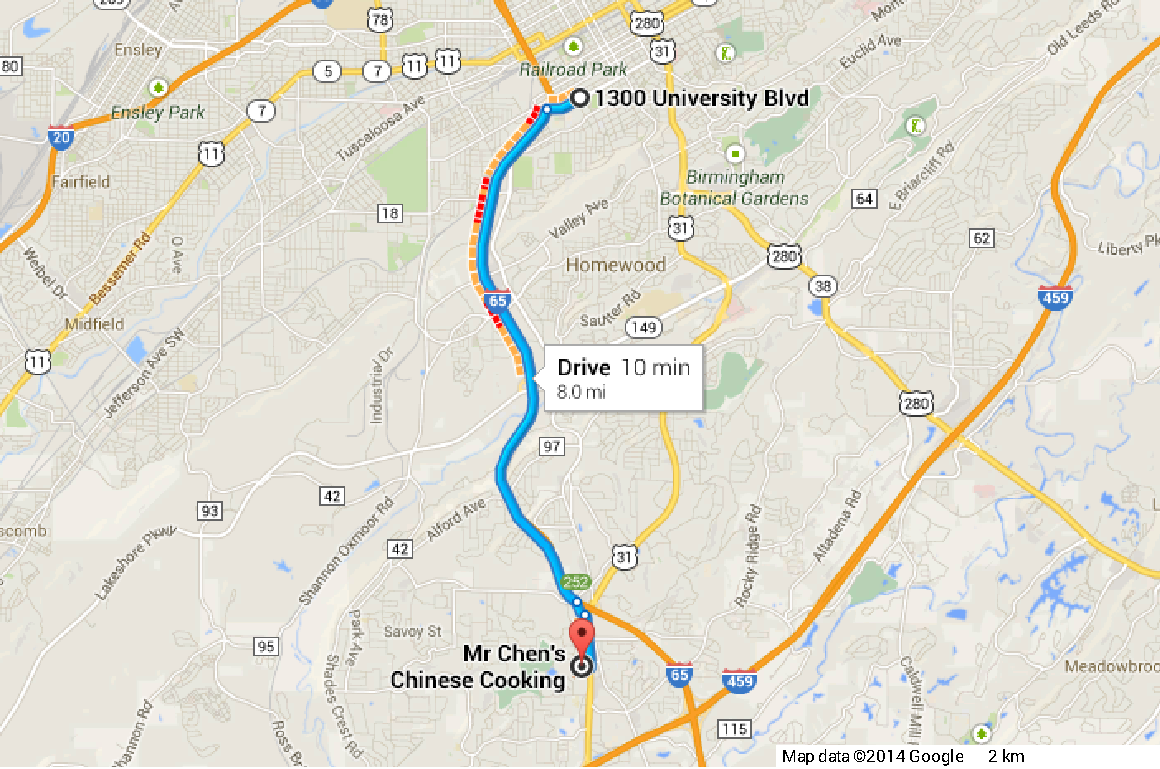
\includegraphics[width=\textwidth]{uab-to-mr-chens.pdf}
	\end{center}
\end{frame}

\begin{frame}{Properties of Search Problems}
	\begin{itemize}
		\item \alert<2->{Fully} or Partially Observable?
		\item \alert<3->{Deterministic} or Stochastic?
		\item Episodic or \alert<4->{Sequential}?
		\item \alert<5->{Static} or Dynamic?
		\item \alert<6->{Discrete} or Continuous?
		\item \alert<7->{Single} or Multi-Agent?
	\end{itemize}
\end{frame}

\begin{frame}{Example: Vacuum Problem}
	\begin{columns}
		\column{.50\textwidth}
			\begin{block}{Problem}
				\begin{itemize}
					\item Start in \searchstate{1}
					\item Left square actions:\\
					      \searchaction{Suck} or \searchaction{Right}
					\item Right square actions:\\
					      \searchaction{Suck} or \searchaction{Left}
					\item Success: \searchstate{7} or \searchstate{8}
					\item Optimal: fewest actions
				\end{itemize}
			\end{block}
			\begin{block}{Solution}<2->
				\uncover<3->{[\searchaction{Suck}, \searchaction{Right}, \searchaction{Suck}]} \\
				\uncover<4->{i.e., [\searchstate{1}, \searchstate{5}, \searchstate{6}, \searchstate{8}]}
			\end{block}
		\column{.50\textwidth}
			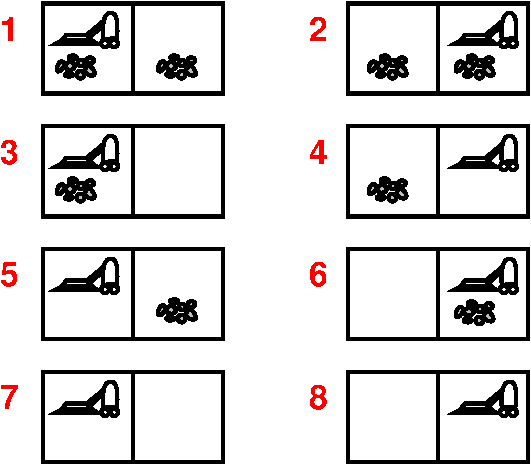
\includegraphics[width=2.1in]{vacuum-space.pdf}
	\end{columns}
\end{frame}

\begin{frame}{Defining a Search Problem}
	\begin{block}{Components}
		\begin{itemize}
			\item Initial state
			\item Actions
			\item Goal test
			\item Path cost
		\end{itemize}
	\end{block}
	\begin{block}{Solution}
		Path from initial state to goal state
	\end{block}
	\begin{block}{Optimal solution}
		Path with lowest cost
	\end{block}
\end{frame}

\begin{frame}{Defining the Vacuum Problem}
	\begin{columns}
		\column{.45\textwidth}
			\begin{block}{Initial State}
				\searchstate{1}
			\end{block}
			\begin{block}{Actions}
				\small
	      $S(\searchstate{1}) = \{(\searchaction{Right}, \searchstate{2}), (\searchaction{Suck}, \searchstate{5})\}$ \\
	      $S(\searchstate{2}) = \{(\searchaction{Left}, \searchstate{1}), (\searchaction{Suck}, \searchstate{4})\}$ \\
	      \ldots
			\end{block}
			\begin{block}{Goal Test}
				$G(s) = s \in \{\searchstate{7}, \searchstate{8}\}$
			\end{block}
			\begin{block}{Path Cost}
				1 per state
			\end{block}
		\column{.50\textwidth}
			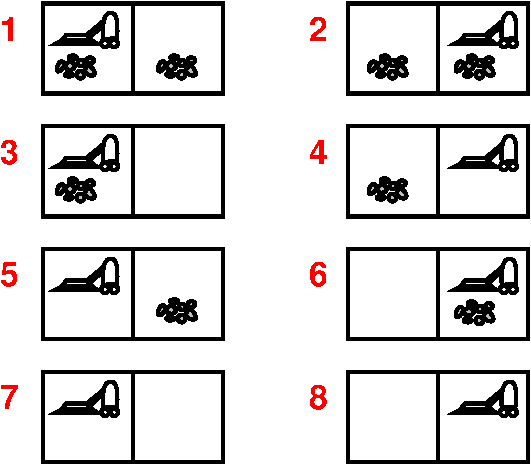
\includegraphics[width=2.1in]{vacuum-space.pdf}
	\end{columns}
\end{frame}

\begin{frame}{Defining the 8-Puzzle Problem}
	\begin{center}
		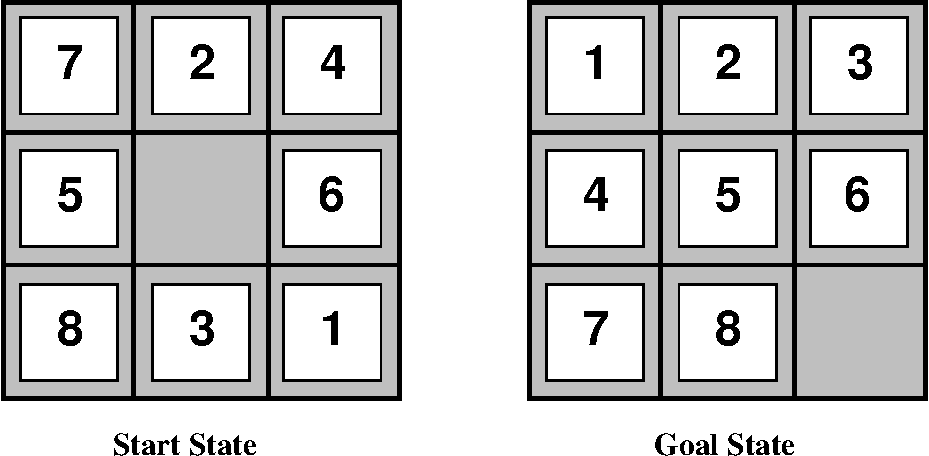
\includegraphics[height=1.5in]{8puzzle.pdf}
	\end{center}
	\begin{description}
		\item[States] \uncover<2->{Mappings of tile numbers to tile locations }
		\item[Initial] \uncover<3->{$\{
			1\!\!:\!\!9,
			2\!\!:\!\!2,
			3\!\!:\!\!8,
			4\!\!:\!\!3,
			5\!\!:\!\!4,
			6\!\!:\!\!6,
			7\!\!:\!\!1,
			8\!\!:\!\!9\}$}
		\item[Actions] \uncover<4->{Move blank left, right, up, down}
		\item[Goal] \uncover<5->{$\{
			1\!\!:\!\!1,
			2\!\!:\!\!2,
			3\!\!:\!\!3,
			4\!\!:\!\!4,
			5\!\!:\!\!5,
			6\!\!:\!\!6,
			7\!\!:\!\!7,
			8\!\!:\!\!8\}$}
		\item[Cost] \uncover<6->{1 per move}
	\end{description}
\end{frame}

\begin{frame}{Defining the Robotic Assembly Problem}
	\begin{center}
		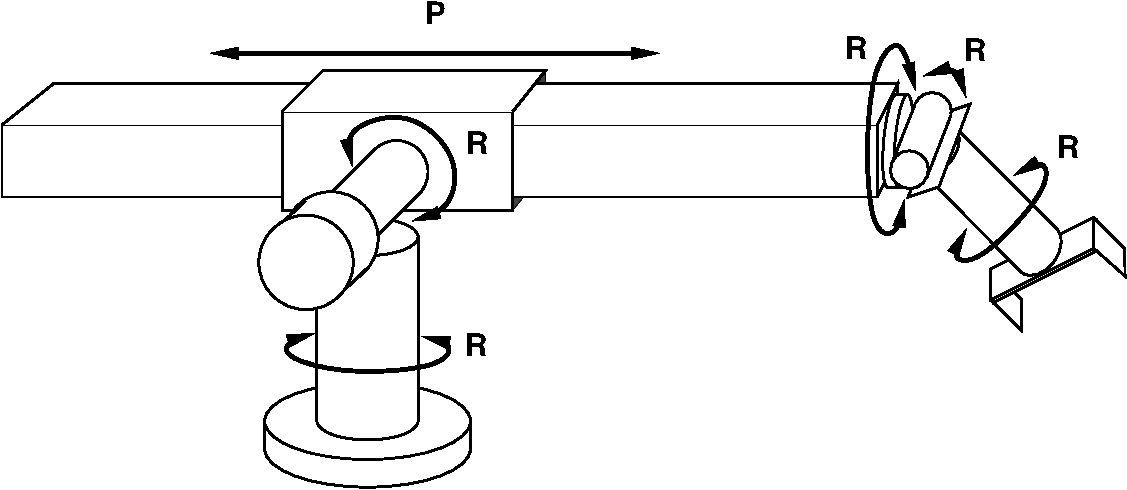
\includegraphics[height=1.5in]{stanford-arm.pdf}
	\end{center}
	\begin{description}
		\item[States] \uncover<2->{real-valued joint angles, parts to assemble}
		\item[Initial] \uncover<3->{many possible}
		\item[Actions] \uncover<4->{real-valued adjustments to joint angles}
		\item[Goal] \uncover<5->{fully assembled part}
		\item[Cost] \uncover<6->{total duration of all movements}
	\end{description}
\end{frame}

\begin{frame}{Defining the Machine Translation Problem}
	\begin{description}
		\item[Input] Com\'i la manzana roja porque ten\'ia hambre.
		\item[Output] I ate the red apple because I was hungry.
		\bigskip\bigskip
		\item[States]
		\item[Initial]
		\item[Actions]
		\item[Goal]
		\item[Cost]
	\end{description}
\end{frame}

\subsection{Search Trees and Search Nodes}

\begin{frame}[fragile]{Tree Search}
	\footnotesize
	\begin{lstlisting}
		def tree_search(problem, strategy):

		    strategy.add(...problem.initial_state...)

		    for node in strategy:

		        if problem.is_goal(node.state):
		            return node.get_actions()

		        items = problem.get_successors(node.state)
		        for state, action, ... in items:
		            strategy.add(...state...action...)

		    return None
	\end{lstlisting}
\end{frame}

\begin{frame}{Search Tree Example}
\begin{center}
\small
\pgfkeys{/pgf/inner sep=0.25em}
\begin{forest}
for tree={grow'=east,l sep=4em}
[Birmingham
  [Atlanta,visible on={2-}
    [Birmingham,visible on={3-}]
    [Chattanooga,visible on={3-}]
    [Augusta,visible on={3-}]
    [\ldots,visible on={3-}]
  ]
  [Montgomery,visible on={2-}
    [Birmingham,visible on={4-}]
    [Atlanta,visible on={4-}]
    [Mobile,visible on={4-}]
    [\ldots,visible on={4-}]
  ]
  [Tuscaloosa,visible on={2-}
    [Birmingham,visible on={5-}]
    [Meridian,visible on={5-}]
    [Starkville,visible on={5-}]
    [\ldots,visible on={5-}]
  ]
]
\end{forest}
\end{center}
\end{frame}

\begin{frame}{The Node Data Structure}
	\begin{center}
		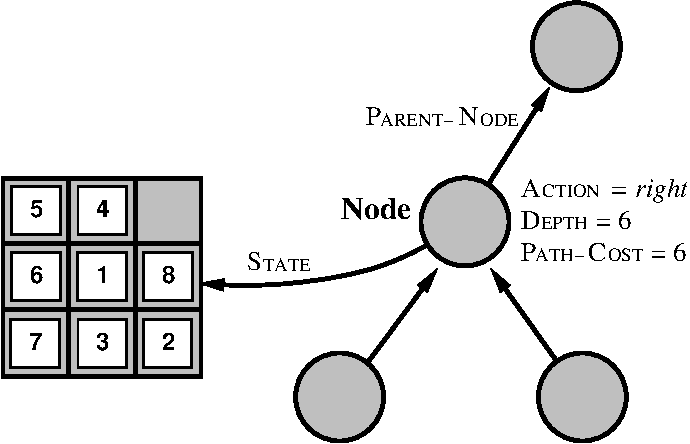
\includegraphics[width=4in]{state-vs-node.pdf}
	\end{center}
\end{frame}

\begin{frame}[fragile]{Tree Search Revisited}
	\footnotesize
	\begin{lstlisting}
		def tree_search(problem, strategy):
		    strategy.add(Node(problem.initial_state))
		    for node in strategy:
		        if problem.is_goal(node.state):
		            return node.get_actions()
		        succs = problem.get_successors(node.state)
		        for state, action, cost in succs:
		            strategy.add(Node(
		                state=state,
		                action=action,
		                parent=node,
		                cost=node.cost + cost,
		                depth=node.depth + 1))
		    return None
	\end{lstlisting}
\end{frame}

\section{Uninformed Search Strategies}
\begin{frame}[<+->]{Search Strategy Properties}
	\begin{block}{Completeness}
		If a solution exists, is it always found?
	\end{block}
	\begin{block}{Optimality}
		Is the solution found always the lowest cost?
	\end{block}
	\begin{block}{Time Complexity}
		How many search nodes will be generated?
	\end{block}
	\begin{block}{Space Complexity}
		How many search nodes must stay in main memory?
	\end{block}
\end{frame}

\subsection{Breadth-first Search}
\begin{frame}[label=breadth-first-example]{Breadth-first Search}
\begin{center}
\begin{forest}
for tree={circle,draw}
[A,visible on filled on={1-}{2-}
  [B,visible on filled on={2-}{3-}
    [D,visible on filled on={3-}{5-}
      [H,visible on={5-}]
      [I,visible on={5-}]
    ]
    [E,visible on filled on={3-}{6-}
      [J,visible on={6-}]
      [K,visible on={6-}]
    ]
  ]
  [C,visible on filled on={2-}{4-}
    [F,visible on filled on={4-}{7-}
      [L,visible on={7-}]
      [M,visible on={7-}]
    ]
    [G,visible on={4-}
      [N,invisible]
      [O,invisible]
    ]
  ]
]
\end{forest}
\end{center}
\end{frame}
\begin{frame}{Breadth-first Properties}
	\footnotesize
	\begin{block}{Strategy? \hyperlink{breadth-first-example}{\beamergotobutton{Example}}}
		 \uncover<2->{First-in First-Out Queue}
	\end{block}
	\begin{block}{Complete?}
		\uncover<3->{Yes, if number of branches is finite}
	\end{block}
	\begin{block}{Optimal?}
		\uncover<4->{Yes, if step costs are all identical}
	\end{block}
	\begin{block}{Worst Case Time Complexity?}
		\uncover<5->{$O(b^{d+1})$, branching factor $b$, depth of goal state $d$}
	\end{block}
	\begin{block}{Worst Case Space Complexity?}
		\uncover<6->{$O(b^{d+1})$, branching factor $b$, depth of goal state $d$}
	\end{block}
\end{frame}

\subsection{Uniform-cost Search}
\begin{frame}[label=uniform-cost-example]{Uniform-cost Search}
\begin{center}
\begin{forest}
for tree={circle,draw},
[A,visible on filled on={1-}{2-}
  [B,edge weight={2},visible on filled on={2-}{4-}
    [D,edge weight={1},visible on filled on={4-}{6-}
      [H,edge weight={2},visible on={6-}]
      [I,edge weight={3},visible on={6-}]
    ]
    [E,edge weight={1},visible on={4-}
      [J,edge weight={3},invisible]
      [K,edge weight={2},invisible]
    ]
  ]
  [C,edge weight={1},visible on filled on={2-}{3-}
    [F,edge weight={3},visible on={3-}
      [L,edge weight={1},invisible]
      [M,edge weight={1},invisible]
    ]
    [G,edge weight={2},visible on filled on={3-}{5-}
      [N,edge weight={1},visible on={5-}]
      [O,edge weight={3},visible on={5-}]
    ]
  ]
]
\end{forest}
\end{center}
\end{frame}
\begin{frame}{Uniform-cost Search}
	\footnotesize
	\begin{block}{Strategy? \hyperlink{uniform-cost-example}{\beamergotobutton{Example}}}
		\uncover<2->{Lowest Cost First Priority Queue}
	\end{block}
	\begin{block}{Complete?}
		\uncover<3->{Yes, if number of branches is finite and steps are all positive}
	\end{block}
	\begin{block}{Optimal?}
		\uncover<4->{Yes}
	\end{block}
	\begin{block}{Worst Case Time Complexity?}
		\uncover<5->{$O(b^{\left\lfloor C^{*}/\epsilon \right\rfloor +1})$, optimal cost $C^{*}$, minimum step cost $\epsilon$}
	\end{block}
	\begin{block}{Worst Case Space Complexity?}
		\uncover<6->{$O(b^{\left\lfloor C^{*}/\epsilon \right\rfloor +1})$, optimal cost $C^{*}$, minimum step cost $\epsilon$}
	\end{block}
\end{frame}

\subsection{Depth-first Search}
\begin{frame}[label=depth-first-example]{Depth-first Search}
\begin{center}
\begin{forest}
for tree={circle,draw}
[A,visible on filled on={1-}{2-}
  [B,visible on filled on={2-9}{3-}
    [D,visible on filled on={3-6}{4-}
      [H,visible on filled on={4-5}{5-}]
      [I,visible on filled on={4-6}{6-}]
    ]
    [E,visible on filled on={3-9}{7-}
      [J,visible on filled on={7-8}{8-}]
      [K,visible on filled on={7-9}{9-}]
    ]
  ]
  [C,visible on={2-10}
    [F,invisible
      [L,invisible]
      [M,invisible]
    ]
    [G,invisible
      [N,invisible]
      [O,invisible]
    ]
  ]
]
\end{forest}
\end{center}
\end{frame}
\begin{frame}{Depth-first Properties}
	\footnotesize
	\begin{block}{Strategy? \hyperlink{depth-first-example}{\beamergotobutton{Example}}}
		\uncover<2->{First-in Last-Out Stack}
	\end{block}
	\begin{block}{Complete?}
		\uncover<3->{Yes, if finite number of states and no cyclic paths}
	\end{block}
	\begin{block}{Optimal?}
		\uncover<4->{No, lower goal states may be found first}
	\end{block}
	\begin{block}{Worst Case Time Complexity?}
		\uncover<5->{$O(b^{m})$, branching factor $b$, maximum depth $m$}
	\end{block}
	\begin{block}{Worst Case Space Complexity?}
		\uncover<6->{$O(bm)$, branching factor $b$, maximum depth $m$}
	\end{block}
\end{frame}

\subsection{Iterative Deepening Search}
\begin{frame}[label=iterative-deepening-example]{Iterative Deepening Search}
\begin{center}
\begin{forest}
for tree={circle,draw}
[A,visible on filled on={1-2,4-7,9-16,18}{2,5-7,10-16}
  [B,visible on filled on={5-6,10-13}{6,11-13}
    [D,visible on filled on={11-12}{12}
      [H,invisible]
      [I,invisible]
    ]
    [E,visible on filled on={11-13}{13}
      [J,invisible]
      [K,invisible]
    ]
  ]
  [C,visible on filled on={5-7,10-16}{7,14-16}
    [F,visible on filled on={14-15}{15}
      [L,invisible]
      [M,invisible]
    ]
    [G,visible on filled on={14-16}{16}
      [N,invisible]
      [O,invisible]
    ]
  ]
]
\end{forest}
\end{center}
\end{frame}
\begin{frame}{Iterative Deepening Properties}
	\footnotesize
	\begin{block}{Strategy? \hyperlink{iterative-deepening-example}{\beamergotobutton{Example}}}
		\uncover<2->{First-in Last-Out Stack with depth limit}
	\end{block}
	\begin{block}{Complete?}
		\uncover<3->{Yes, if number of branches is finite}
	\end{block}
	\begin{block}{Optimal?}
		\uncover<4->{Yes, if step costs are all identical}
	\end{block}
	\begin{block}{Worst Case Time Complexity?}
		\uncover<5->{$O(b^{d})$, branching factor $b$, depth of goal state $d$}
	\end{block}
	\begin{block}{Worst Case Space Complexity?}
		\uncover<6->{$O(bd)$, branching factor $b$, depth of goal state $d$}
	\end{block}
\end{frame}

\subsection*{Repeated States}
\begin{frame}{Exponential Costs of Repeated States}
	\begin{center}
		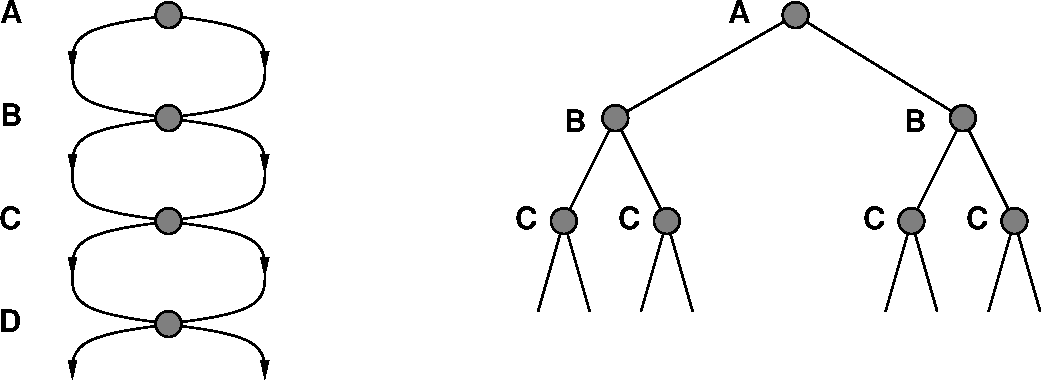
\includegraphics[width=4in]{ribbon-space.pdf}
	\end{center}
\end{frame}
\begin{frame}[fragile]{Graph Search}
	\scriptsize
	\begin{lstlisting}
		def graph_search(problem, strategy):
		    seen = set()
		    strategy.add(Node(problem.initial_state))
		    for node in strategy:
		        if problem.is_goal(node.state):
		            return node.get_actions()
		        if node not in seen:
		            seen.add(node)
		            succs = problem.get_successors(node.state)
		            for state, action, cost in succs:
		                strategy.add(Node(
		                    state=state,
		                    action=action,
		                    parent=node,
		                    cost=node.cost + cost,
		                    depth=node.depth + 1))
	\end{lstlisting}
\end{frame}

\section{Informed Search}
\begin{frame}{All States are not Equal}
	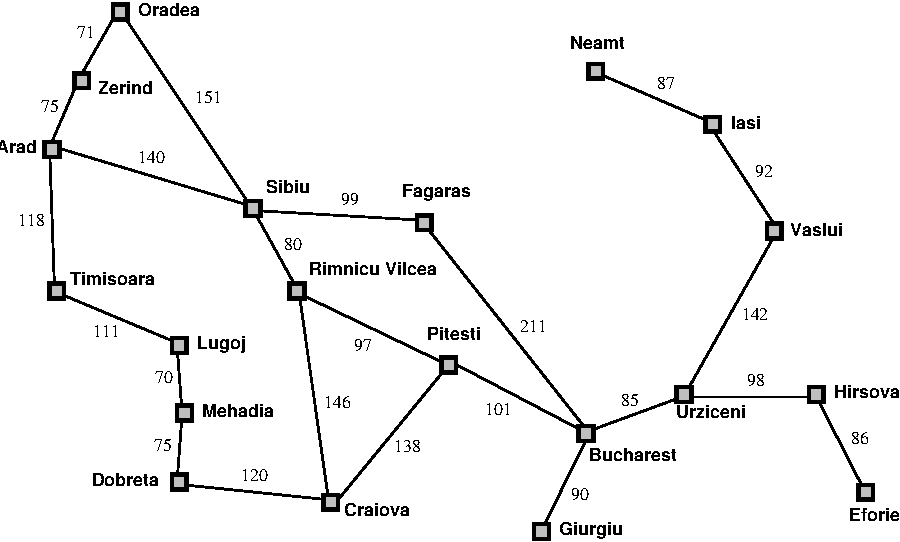
\includegraphics[width=4in]{romania-distances.pdf}
\end{frame}

\subsection{Best-First Search}

\begin{frame}[label=greedy-example]{Best-First (Greedy) Search}
\begin{center}
\footnotesize
\begin{forest}
for tree={draw,rounded corners,align=center}
[{\greedynode{Arad}{366}},visible on filled on={1-}{2-}
  [{\greedynode{Sibiu}{253}},visible on filled on={2-}{3-}
    [{\greedynode{Arad}{366}},visible on={3-}]
    [{\greedynode{Fagaras}{176}},visible on filled on={3-}{4-}
      [{\greedynode{Sibiu}{253}},visible on={4-}]
      [{\greedynode{Bucharest}{0}},visible on filled on={4-}{5-}]
    ]
    [{\greedynode{Oradea}{380}},visible on={3-}]
    [{\greedynode{Rimnicu Vilcea}{193}},visible on={3-}]
  ]
  [{\greedynode{Timisoara}{329}},visible on={2-}]
  [{\greedynode{Zerind}{374}},visible on={2-}]
]
\end{forest}
\end{center}
\end{frame}
\begin{frame}[label=greedy-properties]{Best-First (Greedy) Properties}
	\footnotesize
	\begin{block}{Strategy?}
		 \uncover<2->{Priority Queue, $f(n) = h(n)$}
	\end{block}
	\begin{block}{Complete?}
		\uncover<3->{Yes, if finite number of states and no cyclic paths}
	\end{block}
	\begin{block}{Optimal?}
		\uncover<4->{No}
	\end{block}
	\begin{block}{Worst Case Time Complexity?}
		\uncover<5->{$O(b^m)$, but better with good heuristic}
	\end{block}
	\begin{block}{Worst Case Space Complexity?}
		\uncover<6->{$O(b^m)$}
	\end{block}
\end{frame}

\subsection{A* Search}
\begin{frame}[label=a-star-example]{A* Search}
\begin{center}
\tiny
\begin{forest}
for tree={draw,rounded corners,align=center,l sep=3em}
[{\astarnode{Arad}{0 + 366}{366}},visible on filled on={1-}{2-}
  [{\astarnode{Sibiu}{140+253}{393}},edge weight=140,visible on filled on={2-}{3-}
    [{\astarnode{Arad}{280+366}{646}},edge weight=140,visible on={3-}]
    [{\astarnode{Fagaras}{239+176}{415}},edge weight=99,visible on filled on={3-}{5-}
      [{\astarnode{Sibiu}{338+253}{591}},edge weight=99,visible on={5-}]
      [{\astarnode{Bucharest}{450+0}{450}},edge weight=211,visible on={5-}]
    ]
    [{\astarnode{Oradea}{291+380}{671}},edge weight=151,visible on={3-}]
    [{\astarnode{Rimnicu Vilcea}{220+193}{413}},edge weight=80,visible on filled on={3-}{4-}
      [{\astarnode{Craiova}{366+160}{526}},edge weight=146,visible on={4-}]
      [{\astarnode{Pitesti}{317+100}{417}},edge weight=91,visible on filled on={4-}{6-}
        [{\astarnode{Bucharest}{418+0}{418}},edge weight=101,visible on filled on={6-}{7-}]
        [{\astarnode{Craiova}{455+160}{615}},edge weight=138,visible on={6-}]
        [{\astarnode{Rimnicu Vilcea}{414+193}{607}},edge weight=97,visible on={6-}]
      ]
      [{\astarnode{Sibiu}{300+253}{553}},edge weight=80,visible on={4-}]
    ]
  ]
  [{\astarnode{Timisoara}{118+329}{447}},edge weight=118,visible on={2-}]
  [{\astarnode{Zerind}{75+374}{449}},edge weight=75,visible on={2-}]
]
\end{forest}
\end{center}
\end{frame}
\begin{frame}[label=a-star-properties]{A* Properties}
	\footnotesize
	\begin{block}{Strategy?}
		 \uncover<2->{Priority Queue, $f(n) = g(n) + h(n)$}
	\end{block}
	\begin{block}{Complete?}
		\uncover<3->{Yes, if there are finite nodes with $f(n) < C^{*}$}
	\end{block}
	\begin{block}{Optimal?}
		\uncover<4->{Yes, if $h$ is consistent}
	\end{block}
	\begin{block}{Worst Case Time Complexity?}
		\uncover<5->{All nodes with $f(n) < C^{*}$, exponential in \texttt{len(path)}}
	\end{block}
	\begin{block}{Worst Case Space Complexity?}
		\uncover<6->{All nodes with $f(n) < C^{*}$}
	\end{block}
\end{frame}

\begin{frame}{Proof that A* is Optimal}
	\begin{columns}[T]
		\begin{column}{1.75in}
			Suppose some suboptimal goal $G_2$ has been generated and is in the queue. Let $n$ be an unexpanded node on a shortest path to an optimal goal $G_1$.
		\end{column}
		\begin{column}{2.25in}
			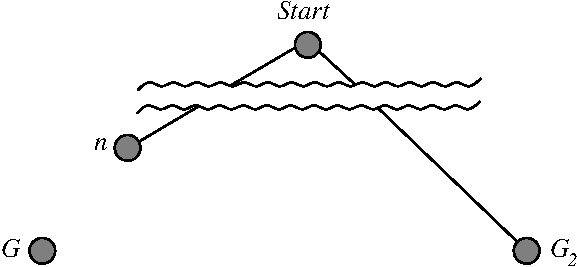
\includegraphics[width=2.25in]{a-star-proof.pdf}
		\end{column}
	\end{columns}
	\bigskip
	\[
	\begin{array}{llll}
	\uncover<2->{f(G_2)} & \uncover<2->{=  }  & \uncover<2->{g(G_2)} & \uncover<2->{\mbox{since $h(G_2) = 0$}} \\
	\uncover<3->{      } & \uncover<3->{>  }  & \uncover<3->{g(G_1)} & \uncover<3->{\mbox{since $G_2$ is suboptimal}} \\
	\uncover<4->{      } & \uncover<4->{\geq} & \uncover<4->{f(n)  } & \uncover<4->{\mbox{since $h$ is consistent}}
	\end{array}
	\]
	\bigskip
	\uncover<5->{Since $f(G_2) > f(n)$, A* will never select $G_2$ for expansion.}
\end{frame}
\begin{frame}{A* Contours}
	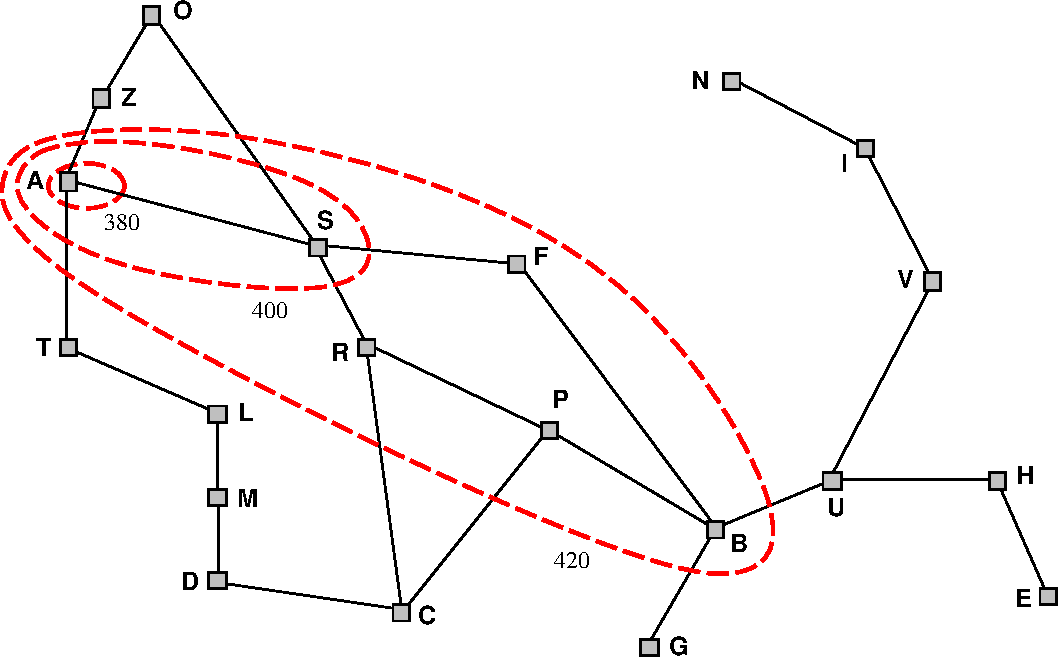
\includegraphics[width=4in]{a-star-contours.pdf}
\end{frame}

\subsection{Heuristic Functions}

\begin{frame}{8-Puzzle Heuristics}
	\begin{center}
		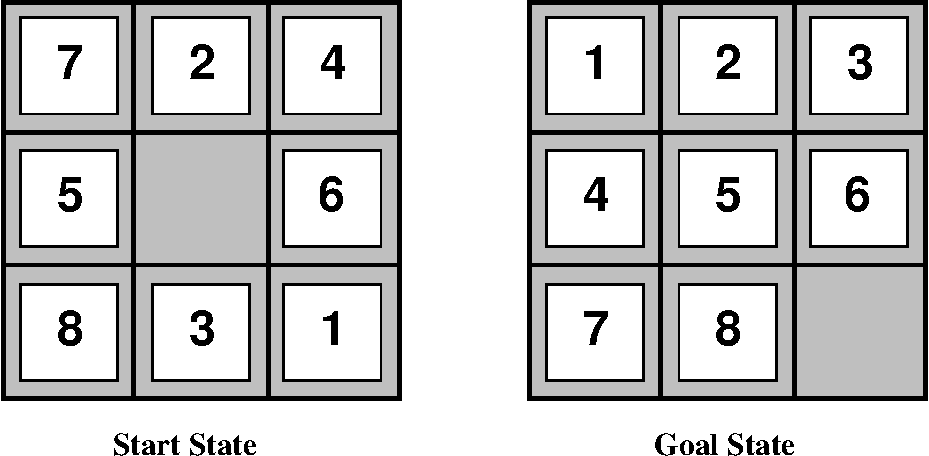
\includegraphics[height=1.25in]{8puzzle.pdf}
	\end{center}
	\begin{tabular}{ll}
		\medskip
		\uncover<2->{\color{blue}Misplaced Tiles}    & \uncover<3->{\footnotesize $h(n) = 6$} \\
		\medskip
		\uncover<4->{\color{blue}Manhattan Distance} & \uncover<5->{\footnotesize $h(n) = 4 + 0 + 3 + 3 + 1 + 0 + 2 + 1$} \\
	\end{tabular}
\end{frame}
\begin{frame}{Heuristic Quality}
	\begin{block}{All heuristics were not created equal}
		\begin{tabular}{rrr}
			                      & \color{blue}Misplaced Tiles & \color{blue}Manhattan Distance \\
			\color{blue} 4 moves  &                    13 nodes &                       12 nodes \\
			\color{blue} 8 moves  &                    39 nodes &                       25 nodes \\
			\color{blue}12 moves  &                   227 nodes &                       73 nodes \\
			\color{blue}16 moves  &                  1301 nodes &                      211 nodes \\
			\color{blue}20 moves  &                  7276 nodes &                      676 nodes \\
		\end{tabular}
	\end{block}
\end{frame}
\begin{frame}{Heuristic Dominance}
	\begin{block}{Dominance}
		$h_1$ \textbf{dominates} $h_2$ if for all $n$, $h_1(n) \geq h_2(n)$
		\\ \bigskip
		Which one dominates?
		\begin{itemize}
			\item Misplaced Tiles
			\item<1-|alert@2-> Manhattan Distance
		\end{itemize}
	\end{block}
	\begin{block}<3->{Dominance = Efficiency}
		A* with $h_1$ will never expand more nodes than A* with $h_2$
		\\ \bigskip
		\alert{Why?} \uncover<4->{Every node with $h(n) < C^{*} - g(n)$ is expanded}
	\end{block}
\end{frame}

\begin{frame}{Relaxed Problems}
	\begin{block}{The 8-Puzzle}
		\begin{tabular}{ll}
			\bf Problem                                  & \bf Heuristic\\
			\hline
			\uncover<2->{Tiles move anywhere}            & \uncover<3->{Misplaced Tiles} \\
			\uncover<4->{Tiles move to adjacent squares} & \uncover<5->{Manhattan Distance} \\
		\end{tabular}
	\end{block}
	
	\begin{block}<6->{Generating heuristics}
		Exact solution to relaxed problem $\Rightarrow$ consistent heuristic
		\\ \bigskip
		\alert{Why?}
		\uncover<7->{
		\begin{itemize}
			\item Solution in original problem is also solution in relaxed
			\item Heuristic is exact cost in relaxed $\Rightarrow$ triangle inequality
		\end{itemize}
		}
	\end{block}
\end{frame}

\begin{frame}{Traveling Salesman Problem}
	\begin{columns}
		\begin{column}{2in}
			\begin{block}{Problem}
				Visit all cities exactly once, minimum distance
			\end{block}
			\begin{center}
				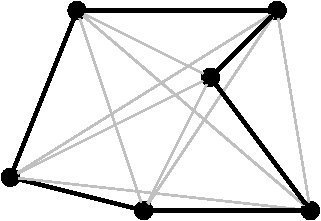
\includegraphics[width=2in]{tsp.pdf}
			\end{center}
		\end{column}
		\pause
		\begin{column}{2in}
			\begin{block}{Heuristic}
				Minimum spanning tree \\
				Solvable in $O(n^2)$
			\end{block}
			\begin{center}
				\visible<2>{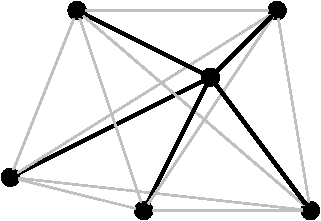
\includegraphics[width=2in]{mst.pdf}}%
			\end{center}
		\end{column}
	\end{columns}
\end{frame}
\begin{frame}[label=bag-generation]{Bag Generation}
\vspace{-1em}
\begin{columns}[t]
\begin{column}{0.7\textwidth}
\begin{block}{Order of a bag of words}
\begin{description}[Actions]
\item[Initial] Full bag, empty sentence
\item[Actions] Pop from bag, add to sentence
\item[Goal] Empty bag, full sentence
\item[Cost] \footnotesize $c(w_1,w_2) + c(w_2,w_3) + \ldots + c(w_{n-1},w_n)$
\end{description}
\end{block}
\end{column}
\begin{column}{0.25\textwidth}
\small
\begin{block}{$c(v,w)$}
\begin{tabular}{@{} l @{\hspace{0.5em}} l @{\hspace{0.5em}} r @{}}
\ldots \\
John & broke & 3.5 \\
\ldots \\
the & the & 25.1 \\
\dots
\end{tabular}
\end{block}
\end{column}
\end{columns}
\smallskip
\centering
\scriptsize
\begin{forest}
for tree={draw,rounded corners,grow'=east,edge=-latex,l sep=2em}
[{\mtnode{lamp,John,the,broke}{}}
  [{\mtnode{lamp,John,broke}{the}}
    [{\mtnode{lamp,broke}{the,John}}
      [{\ldots},draw=none
        [{\mtnode{}{the,John,lamp,broke}}]
      ]
    ]
    [{\mtnode{John,broke}{the,lamp}}
      [{\ldots},draw=none]
    ]
  ]
  [{\mtnode{lamp,the,broke}{John}}
    [{\mtnode{lamp,the}{John,broke}}
      [{\ldots},draw=none
        [{\mtnode{}{John,broke,the,lamp}}]
      ]
    ]
    [{\mtnode{lamp,broke}{John,the}}
      [{\ldots},draw=none]
    ]
  ]
]
\end{forest}
\end{frame}
\begin{frame}[label=bag-generation-heuristic]{A Bag Generation Heuristic}
\begin{columns}
\begin{column}{0.6\textwidth}
\begin{block}{Node}
\texttt{$\{$lamp, the$\}$} \\
\texttt{[John, broke]}
\end{block}
\begin{block}{Bag-Word Estimates}
$
\begin{array}{@{} l l @{}}
\alt<2->%
{\min\limits_{w \in \{\mbox{\scriptsize broke}, \mbox{\scriptsize the}\}} s(w, \mbox{lamp})}
{\mbox{lamp}}
& \uncover<3->{3.5} \\
\alt<2->%
{\min\limits_{w \in \{\mbox{\scriptsize broke}, \mbox{\scriptsize lamp}\}} s(w, \mbox{the})}
{\mbox{the}}
& \uncover<4->{3.2} \\
\end{array}
$
\end{block}
\begin{block}{h(n)}
\uncover<5->{$3.5 + 3.2 = 6.7$}
\end{block}
\end{column}
\begin{column}{0.35\textwidth}
\begin{tabular}{ @{} | l l r | @{}}
\hline
John  & lamp & 7.6 \\
broke & lamp & 6.9 \\
the   & lamp & 3.5 \\
lamp  & lamp & 23.0 \\
\hline
\hline
John  & the  & 7.1 \\
broke & the  & 3.2 \\
the   & the  & 25.1 \\
lamp  & the  & 6.2 \\
\hline
\end{tabular}
\end{column}
\end{columns}
\end{frame}


\part{Key Points}
\begin{frame}[label=key-points]{Key Points}
	\begin{block}{Search Problems}
		\begin{itemize}
			\item Initial State, Actions, Goal Test, Path Cost
		\end{itemize}
	\end{block}
	\begin{block}{Search Strategies}
		\begin{itemize}
			\item Breadth-first
			\item Uniform-cost
			\item Depth-first
			\item Iterative Deepening
			\item A* Search
		\end{itemize}
	\end{block}
	\begin{block}{Heuristics}
		\begin{itemize}
			\item Dominance, Relaxed Problems
		\end{itemize}
	\end{block}
\end{frame}


\end{document}


